\documentclass{beamer}
\usepackage{amsmath}
\usepackage[english]{babel} %set language; note: after changing this, you need to delete all auxiliary files to recompile
\usepackage[utf8]{inputenc} %define file encoding; latin1 is the other often used option
\usepackage{csquotes} % provides context sensitive quotation facilities
\usepackage{graphicx} %allows for inserting figures
\usepackage{booktabs} % for table formatting without vertical lines
\usepackage{textcomp} % allow for example using the Euro sign with \texteuro
\usepackage{stackengine}
\usepackage{wasysym}
\usepackage{tikzsymbols}
\usepackage{textcomp}
\usetikzlibrary{patterns} 
\usepackage{xcolor}
\usepackage[dvipsnames]{xcolor}
\usepackage{colortbl}
\usepackage{adjustbox}
\usetikzlibrary{decorations}
\usetikzlibrary{decorations.pathreplacing}
\usetikzlibrary{decorations.markings}
\newcommand{\bubblethis}[2]{
        \tikz[remember picture,baseline]{\node[anchor=base,inner sep=0,outer sep=0]%
        (#1) {\underline{#1}};\node[overlay,cloud callout,callout relative pointer={(0.2cm,-0.7cm)},%
        aspect=2.5,fill=yellow!90] at ($(#1.north)+(-0.5cm,1.6cm)$) {#2};}%
    }%
\tikzset{face/.style={shape=circle,minimum size=4ex,shading=radial,outer sep=0pt,
        inner color=white!50!yellow,outer color= yellow!70!orange}}
%% Some commands to make the code easier
\newcommand{\emoticon}[1][]{%
  \node[face,#1] (emoticon) {};
  %% The eyes are fixed.
  \draw[fill=white] (-1ex,0ex) ..controls (-0.5ex,0.2ex)and(0.5ex,0.2ex)..
        (1ex,0.0ex) ..controls ( 1.5ex,1.5ex)and( 0.2ex,1.7ex)..
        (0ex,0.4ex) ..controls (-0.2ex,1.7ex)and(-1.5ex,1.5ex)..
        (-1ex,0ex)--cycle;}
\newcommand{\pupils}{
  %% standard pupils
  \fill[shift={(0.5ex,0.5ex)},rotate=80] 
       (0,0) ellipse (0.3ex and 0.15ex);
  \fill[shift={(-0.5ex,0.5ex)},rotate=100] 
       (0,0) ellipse (0.3ex and 0.15ex);}

\newcommand{\emoticonname}[1]{
  \node[below=1ex of emoticon,font=\footnotesize,
        minimum width=4cm]{#1};}
\usepackage{scalerel}
\usetikzlibrary{positioning}
\usepackage{xcolor,amssymb}
\newcommand\dangersignb[1][2ex]{%
  \scaleto{\stackengine{0.3pt}{\scalebox{1.1}[.9]{%
  \color{red}$\blacktriangle$}}{\tiny\bfseries !}{O}{c}{F}{F}{L}}{#1}%
}
\newcommand\dangersignw[1][2ex]{%
  \scaleto{\stackengine{0.3pt}{\scalebox{1.1}[.9]{%
  \color{red}$\blacktriangle$}}{\color{white}\tiny\bfseries !}{O}{c}{F}{F}{L}}{#1}%
}
\usepackage{fontawesome} % Social Icons
\usepackage{epstopdf} % allow embedding eps-figures
\usepackage{tikz} % allows drawing figures
\usepackage{amsmath,amssymb,amsthm} %advanced math facilities
\usepackage{lmodern} %uses font that support italic and bold at the same time
\usepackage{hyperref}
\usepackage{tikz}

\usepackage{tcolorbox}

\usefonttheme[onlymath]{serif} %set math font to serif ones

\definecolor{beamerblue}{rgb}{0.2,0.2,0.7} %define beamerblue color for later use

%%% defines highlight command to set text blue
\newcommand{\highlight}[1]{{\color{blue}{#1}}}


%%%%%%% commands defining backup slides so that frame numbering is correct

\newcommand{\backupbegin}{
   \newcounter{framenumberappendix}
   \setcounter{framenumberappendix}{\value{framenumber}}
}
\newcommand{\backupend}{
   \addtocounter{framenumberappendix}{-\value{framenumber}}
   \addtocounter{framenumber}{\value{framenumberappendix}}
}

%%%% end of defining backup slides

%Specify figure caption, see also http://tex.stackexchange.com/questions/155738/caption-package-not-working-with-beamer
\setbeamertemplate{caption}{\insertcaption} %redefines caption to remove label "Figure".
%\setbeamerfont{caption}{size=\scriptsize,shape=\itshape,series=\bfseries} %sets figure  caption bold and italic and makes it smaller


\usetheme{Boadilla}

\newtcolorbox{boxA}{
    fontupper = \bf,
    boxrule = 1.5pt,
    colframe = black % frame color
}
\newtcolorbox{boxB}{
    boxrule = 1.5pt,
    colframe = blue!70!black,, % frame color
    colback = blue!7!white,
}
% --------------------
% Overall information
% --------------------

\title[Economía I]{Economía I \vspace{4mm}
\\ Magistral 15 y 16: Distorsiones al equilibrio competitivo}
\date{}
\author[Franco Riottini]{Riottini Franco}
\vspace{0.4cm}
\institute[]{Universidad de San Andrés} 

\begin{document}

\begin{frame}
\titlepage
\centering
\includegraphics[scale=0.2]{../Figures/logoUDESA.jpg} 
\end{frame}

\begin{frame}{Distorsiones al equilibrio de mercado}
    En muchas ocasiones el mercado no funciona tan perfectamente. Puede haber dos tipos de distorsiones:
    \begin{itemize}
        \item Creadas por el hombre:
        \begin{itemize}
            \item Monopolios artificiales (escribanos, low cost, SUBE)
            \vspace{1mm}
            \item \only<1>{Impuestos} \only<2->{\textbf{Impuestos}}
            \vspace{1mm}
            \item Precios máximos o mínimos (cepo, "Precios Justos")
            \vspace{1mm}
            \item Regulación (ley de alquileres)
        \end{itemize}
        \vspace{1mm}
        \item Por las características de la realidad:
        \begin{itemize}
            \item Monopolios naturales (red eléctrica, agua, gas)   
            \vspace{1mm}
            \item Externalidades (vacunación, contaminación)
            \vspace{1mm}
            \item Bienes públicos
            \vspace{1mm}
            \item Problemas de información
            \begin{itemize}
                \item Atributos ocultos (selección adversa)
                \vspace{1mm}
                \item Acciones ocultas (moral hazard o riesgo moral)
            \end{itemize}        
        \end{itemize}
    \end{itemize}
\end{frame}

\begin{frame}{El impacto de los impuestos}
    \begin{itemize}
        \item ¿Qué es un impuesto?
        \item Es un tributo generalmente establecido por el Estado
        \begin{itemize}
            \item Para financiar sus gastos
            \item Para ‘guiar’ el comportamiento (por ejemplo en el caso de externalidades)
        \end{itemize}
        \item Existen diversos tipos:
        \begin{itemize}
            \item Al consumo, al trabajo, al ingreso, a la propiedad, etc.
        \end{itemize}
        \item Un impuesto aumentará el precio que los consumidores pagan sobre un bien...
        \item La elasticidad precio de la demanda tendrá influencia sobre el efecto del impuesto
    \end{itemize}
\end{frame}

\begin{frame}{Impuestos y eficiencia}
    \begin{itemize}
        \item La introducción de impuestos aleja a la economía del equilibrio competitivo. 
        \begin{itemize}
            \item Los impuestos sobre oferentes/consumidores desplazan la curva de oferta/demanda porque el precio es más alto para cada cantidad.
            \item Al recaudar impuestos el Estado genera una pérdida de peso muerto. 
        \end{itemize}
        \item ¿Hay que gravar a todos los bienes por igual?
        \begin{itemize}
            \item Si queremos minimizar esa pérdida de peso muerto, deberemos analizar la elasticidad de la demanda de los distintos bienes.
        \end{itemize}
        \item  ¿Sobre quién debería recaer el pago de cada impuesto, consumidores o vendedores? Hay que analizar la incidencia de los impuestos.
        \begin{itemize}
            \item La recaudación se extrae del excedente de consumidores y productores.
            \item La incidencia del impuesto depende de la elasticidad relativa de consumidores y productores.
            \item El grupo menos elástico lleva más de la carga fiscal. 
        \end{itemize}
    \end{itemize}
\end{frame}

\begin{frame}{Impacto de un impuesto a los vendedores}
    \begin{itemize}
        \item Si se impone un impuesto $t$ sobre las cantidades \textbf{vendidas}, la curva de la oferta se ``desplaza'' hacia arriba (izquierda) en una cantidad igual al monto del impuesto.
        \item Esto es porque el impuesto encarece los costos del productor. 
        \item La intersección de la oferta con impuesto y la demanda define el precio que pagarán los consumidores ($P_C$) y la cantidad que se intercambiará en el mercado ($Q_t$).
        \item Pero ojo! Ese precio no es el que reciben los productores, porque incluye el impuesto! El precio del productor ($P_P$) se define como:
          \[ P_P=P_C\ - \ t\] 
        \item El Estado se lleva como recaudación el monto del impuesto por la cantidad que ahora se intercambia: \\
        \begin{center}
              Recaudación = $t \cdot Q_t $ 
        \end{center}
    
    \end{itemize}
\end{frame}
    

\begin{frame}{Incidencia de un impuesto a los vendedores}
    \begin{figure} [H]
    \centering
    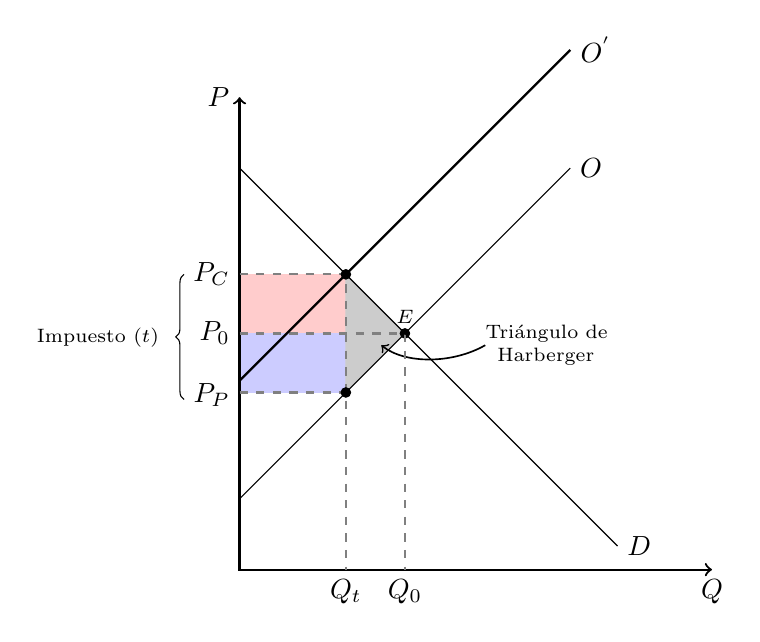
\begin{tikzpicture}[scale=0.6]
    \draw[fill,red!20] (2.25,6.25) rectangle (0,5);
    \draw[fill,blue!20] (0,3.75) rectangle (2.25,5);
    \draw[fill,black!20] (3.5,5)--(2.25,3.75)--(2.25,6.25);
    \node [right] at (5,5) {\scriptsize Triángulo de};
    \node [right] at (5.25,4.5) {\scriptsize Harberger};
    \draw[semithick, <-] (3,4.75)..controls (3.5,4.35) and (4.5,4.35)..(5.2,4.75);
    
    \draw[thick,<->] (0,10) node[left]{$P$}--(0,0)--(10,0) node[below]{$Q$};
    %\node [below left] at (0,0) {$0$};
    \node [below] at (3.5,0) {{$Q_0$}};
    \draw[fill] (3.5,5) circle [radius =0.1] node[above] {\scriptsize $E$};
    \node [left] at (0,5) {$P_0$};
    \node [left] at (0,3.7) {$P_P$};
    \node [left] at (0,6.25) {$P_C$};
    \node [below] at (2.25,0) {{$Q_t$}};
    %\node [below] at (5.25,0) {150};
    \draw[thick,gray, dashed](0,6.25)--(2.25,6.25)--(2.25,0);
    \draw[thick,gray, dashed](0,3.75)--(2.25,3.75);
    
    \draw [thin,decorate,decoration={brace,amplitude=3pt},xshift=5pt,yshift=0pt](-1.35,3.6) -- (-1.35,6.25);
    \draw (-1.5,4.9) node[left]{{\scriptsize Impuesto ($t$)}};
    
    \draw[fill] (2.25,6.25) circle [radius =0.1] ;
    \draw[fill] (2.25,3.75) circle [radius =0.1] ;
    \draw[thick,gray, dashed](0,5)--(3.5,5)--(3.5,0);
    \draw[thin](0,8.5)--(8,0.5) node[right] {$D$};
    \draw[black, domain=0:7] plot (\x, {1.5+\x}) node[right] {$O$};
    
    \draw[thick](0,4)--(7,11) node[right] {$O^{'}$};
    \end{tikzpicture}
    \end{figure} 
\end{frame}

\begin{frame}{Impacto de un impuesto a los vendedores}
    \begin{itemize}
        \item Vemos que, aunque el impuesto se impone sobre los productores, la carga del impuesto se reparte entre consumidores y vendedores. \vspace{2mm}
        \item El Triángulo de Harberger ilustra la pérdida de eficiencia. Entre el segmento $Q_t$ y $Q^*$, la sociedad valora el bien por encima del costo marginal de producción, por lo que esas unidades deberían producirse, pero por el impuesto no sucede. \vspace{2mm}
        \item Ambas cosas (la carga del impuesto y la pérdida de peso muerto) dependen de la elasticidad de la demanda.
    \end{itemize}
\end{frame}

\begin{frame}{Impuestos y elasticidad}
    \begin{itemize}
        \item Un impuesto puede reducir mucho las ventas si su demanda es altamente elástica.
        \begin{itemize}
            \item ¡Y eso puede ser lo que el gobierno intenta hacer!
            \item Por ejemplo, impuestos sobre bienes ‘malos’ para la sociedad como el tabaco o el alcohol o por contaminar.
        \end{itemize}
        \vspace{1mm}
        \item Pero si un impuesto causa una importante caída en las ventas, también reduce los ingresos del impuesto. Por lo tanto, si un gobierno desea aumentar estos ingresos, debería elegir gravar productos con demanda inelástica. 
        \vspace{1mm}
        \item Además, esto permite minimizar la pérdida de peso muerto. Los impuestos deberían ser inversamente proporcionales a la elasticidad de la demanda.
            \begin{itemize}
            \item Si la demanda es totalmente inelástica, no hay pérdida de eficiencia. 
            \end{itemize}
        \begin{boxB}
        \centering
        \small
        Mayor elasticidad de la demanda $\Longrightarrow$ Mayor pérdida de eficiencia \\
        Mayor elasticidad de la demanda $\Longrightarrow$ Menor debería ser el impuesto
        \end{boxB}
    \end{itemize}
\end{frame}

\begin{frame}{Impuestos con demanda perfectamente inelástica}

    \begin{figure} [H]
        \centering
    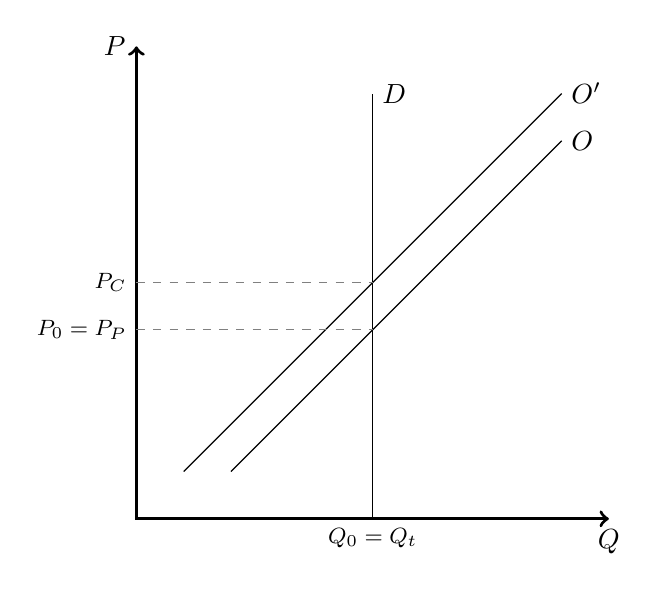
\begin{tikzpicture}[scale=0.6]
    \draw[ very thick,<->] (0,10) node[left]{$P$}--(0,0)--(10,0) node[below]{$Q$};
    %\node [below left] at (0,0) {$0$};
    \draw[thin](1,1)--(9,9) node[right]{$O'$};
    \draw[thin](2,1)--(9,8) node[right]{$O$};
    \draw[thin](5,0)--(5,9) node[right]{$D$};
    \draw[thin,dashed,gray](0,4)--(5,4);
    \draw[thin,dashed,gray](0,5)--(5,5);
    \node[left]at (0,4){\footnotesize $P_0=P_P$};
    \node[left]at (0,5){\footnotesize $P_C$};
    \node[below]at (5,0){\footnotesize $Q_0=Q_t$};
    
    \end{tikzpicture}
    \end{figure} 
\end{frame}

\begin{frame}{Incidencia y elasticidad}
    \begin{itemize}
        \item ¿Quién paga los impuestos? La incidencia también estará determinada por las elasticidades de la oferta y la demanda. 
        \item Tenemos que ver cuanto del impuesto \textbf{puede} trasladar el oferente al demandante.
        \item Independientemente de a quien se le cobra legalmente el impuesto, la carga siempre se reparte (excepto en casos extremos)
            \begin{itemize}
                \item El que tenga mayor elasticidad paga una proporción menor del impuesto
                \item Si la oferta es más elástica que la demanda, los consumidores afrontan mayor proporción del impuesto porque los productores son muy sensibles a caídas en el precio que reciben, por lo que los consumidores estan dispuestos a afrontar una mayor parte del impuesto con tal de no disminuir tanto su consumo.
                \item Si la demanda es más elástica que la oferta, es difícil hacerle pagar el impuesto al consumidor, así que el productor asume más carga.
            \end{itemize}
        \begin{boxB}
        \small
        \centering
        Demanda más elástica que oferta  $\Longrightarrow$ Consumidores pagan menor \% \\
        Oferta más elástica que demanda  $\Longrightarrow$ Productores pagan menor \%
        \end{boxB}
    \end{itemize}
\end{frame}

\begin{frame}{¿Qué pasa con un impuesto a los consumidores?}
    \begin{itemize}
        \item Si se impone un impuesto $t$ sobre las cantidades \textbf{consumidas}, la curva de la demanda se ``desplaza'' hacia abajo (izquierda) en una cantidad igual al monto del impuesto.
        \item Esto es porque, para cualquier cantidad, ahora el consumidor está dispuesto a pagar menos al productor, ya que debe cubrir el impuesto.
        \item La intersección de la demanda con impuesto y la oferta define el precio que recibirán los productores ($P_P$) y la cantidad que se intercambiará en el mercado ($Q_t$).
        \item Pero el precio que pagan los consumidores tiene que tener sumado el impuesto! El precio del consumidor ($P_C$) se define como:
          \[ P_C=P_P\ + \ t\] 
          \vspace{-8mm}
         \item La incidencia será la misma que un impuesto a las cantidades vendidas, pues vimos que esto depende de las elasticidades y no de sobre quién recae legalmente el impuesto. 
    \end{itemize}
\end{frame}

\begin{frame}{Incidencia de un impuesto a los consumidores}
    \begin{figure} [H]
    \centering
    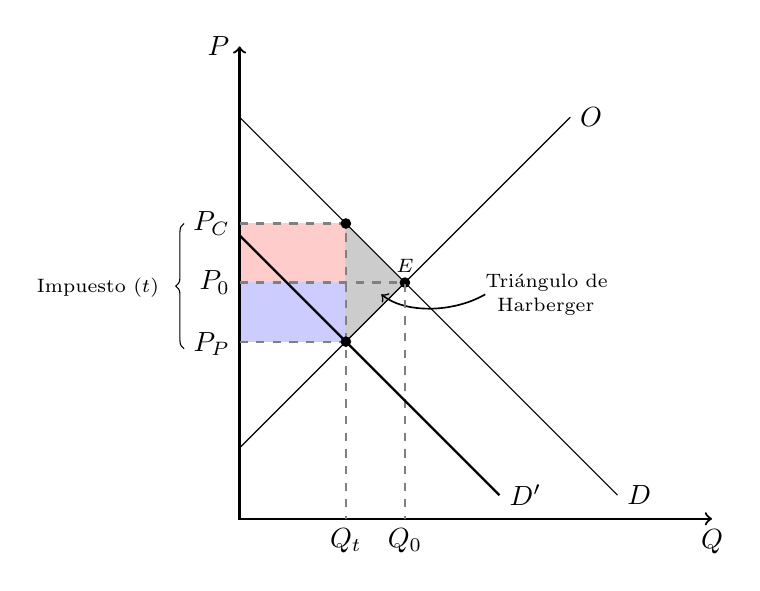
\begin{tikzpicture}[scale=0.6]
    \draw[fill,red!20] (2.25,6.25) rectangle (0,5);
    \draw[fill,blue!20] (0,3.75) rectangle (2.25,5);
    \draw[fill,black!20] (3.5,5)--(2.25,3.75)--(2.25,6.25);
    \node [right] at (5,5) {\scriptsize Triángulo de};
    \node [right] at (5.25,4.5) {\scriptsize Harberger};
    \draw[semithick, <-] (3,4.75)..controls (3.5,4.35) and (4.5,4.35)..(5.2,4.75);
    
    \draw[thick,<->] (0,10) node[left]{$P$}--(0,0)--(10,0) node[below]{$Q$};
    
    \node [below] at (3.5,0) {{$Q_0$}};
    \draw[fill] (3.5,5) circle [radius =0.1] node[above] {\scriptsize $E$};
    \node [left] at (0,5) {$P_0$};
    \node [left] at (0,3.7) {$P_P$};
    \node [left] at (0,6.25) {$P_C$};
    \node [below] at (2.25,0) {{$Q_t$}};
    
    \draw[thick,gray, dashed](0,6.25)--(2.25,6.25)--(2.25,0);
    \draw[thick,gray, dashed](0,3.75)--(2.25,3.75);
    
    \draw [thin,decorate,decoration={brace,amplitude=3pt},xshift=5pt,yshift=0pt](-1.35,3.6) -- (-1.35,6.25);
    \draw (-1.5,4.9) node[left]{{\scriptsize Impuesto ($t$)}};
    
    \draw[fill] (2.25,6.25) circle [radius =0.1] ;
    \draw[fill] (2.25,3.75) circle [radius =0.1] ;
    \draw[thick,gray, dashed](0,5)--(3.5,5)--(3.5,0);
    \draw[thin](0,8.5)--(8,0.5) node[right] {$D$};
    \draw[thick](0,6)--(5.5,0.5) node[right] {$D'$};
    \draw[black, domain=0:7] plot (\x, {1.5+\x}) node[right] {$O$};
    
    \end{tikzpicture}
    \end{figure} 
\end{frame}

\begin{frame}{Comparando impuesto a los vendedores y consumidores}
    
    \begin{columns}
    \begin{column}{0.47\textwidth}
    \centering
    {\small Impuesto a vendedores}
    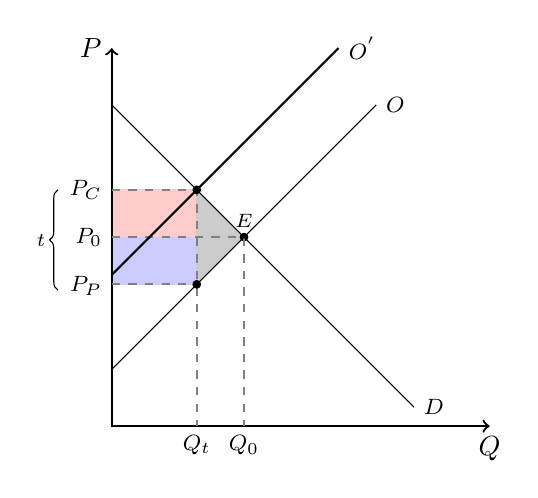
\begin{tikzpicture}[scale=0.48]
    \draw[fill,red!20] (2.25,6.25) rectangle (0,5);
    \draw[fill,blue!20] (0,3.75) rectangle (2.25,5);
    \draw[fill,black!20] (3.5,5)--(2.25,3.75)--(2.25,6.25);
    
    \draw[thick,<->] (0,10) node[left]{$P$}--(0,0)--(10,0) node[below]{$Q$};
    
    \node [below] at (3.5,0) {{\footnotesize $Q_0$}};
    \draw[fill] (3.5,5) circle [radius =0.1] node[above] {\scriptsize $E$};
    \node [left] at (0,5) {\footnotesize $P_0$};
    \node [left] at (0,3.7) {\footnotesize $P_P$};
    \node [left] at (0,6.25) {\footnotesize $P_C$};
    \node [below] at (2.25,0) {\footnotesize {\footnotesize $Q_t$}};
    
    \draw[thick,gray, dashed](0,6.25)--(2.25,6.25)--(2.25,0);
    \draw[thick,gray, dashed](0,3.75)--(2.25,3.75);
    
    \draw [thin,decorate,decoration={brace,amplitude=3pt},xshift=5pt,yshift=0pt](-1.6,3.6) -- (-1.6,6.25);
    \draw (-1.5,4.9) node[left]{{\scriptsize $t$}};
    
    \draw[fill] (2.25,6.25) circle [radius =0.1] ;
    \draw[fill] (2.25,3.75) circle [radius =0.1] ;
    \draw[thick,gray, dashed](0,5)--(3.5,5)--(3.5,0);
    \draw[thin](0,8.5)--(8,0.5) node[right] {\footnotesize $D$};
    \draw[black, domain=0:7] plot (\x, {1.5+\x}) node[right] {\footnotesize $O$};
    
    \draw[thick](0,4)--(6,10) node[right] {\footnotesize $O^{'}$};
    \end{tikzpicture}
    \end{column}
    
    \hfill
    
    \begin{column}{0.49\textwidth}
    \centering
    {\small Impuesto a consumidores}
    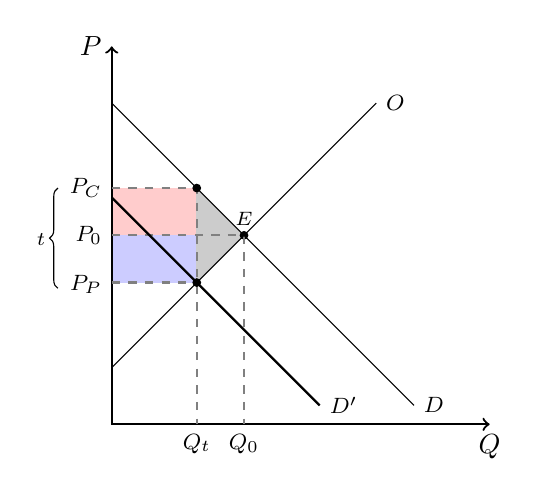
\begin{tikzpicture}[scale=0.48]
    \draw[fill,red!20] (2.25,6.25) rectangle (0,5);
    \draw[fill,blue!20] (0,3.75) rectangle (2.25,5);
    \draw[fill,black!20] (3.5,5)--(2.25,3.75)--(2.25,6.25);
    
    \draw[thick,<->] (0,10) node[left]{$P$}--(0,0)--(10,0) node[below]{$Q$};
    
    \node [below] at (3.5,0) {\footnotesize $Q_0$};
    \draw[fill] (3.5,5) circle [radius =0.1] node[above] {\scriptsize $E$};
    \node [left] at (0,5) {\footnotesize$P_0$};
    \node [left] at (0,3.7) {\footnotesize$P_P$};
    \node [left] at (0,6.25) {\footnotesize$P_C$};
    \node [below] at (2.25,0) {\footnotesize{$Q_t$}};
    
    \draw[thick,gray, dashed](0,6.25)--(2.25,6.25)--(2.25,0);
    \draw[thick,gray, dashed](0,3.75)--(2.25,3.75);
    
    \draw [thin,decorate,decoration={brace,amplitude=3pt},xshift=5pt,yshift=0pt](-1.6,3.6) -- (-1.6,6.25);
    \draw (-1.5,4.9) node[left]{{\scriptsize $t$}};
    
    \draw[fill] (2.25,6.25) circle [radius =0.1] ;
    \draw[fill] (2.25,3.75) circle [radius =0.1] ;
    \draw[thick,gray, dashed](0,5)--(3.5,5)--(3.5,0);
    \draw[thin](0,8.5)--(8,0.5) node[right] {\footnotesize $D$};
    \draw[thick](0,6)--(5.5,0.5) node[right] {\footnotesize $D'$};
    \draw[black, domain=0:7] plot (\x, {1.5+\x}) node[right] {\footnotesize$O$};
    
    \end{tikzpicture}
    
    \end{column}
    \end{columns}
\end{frame}

\begin{frame}{Veamos un ejemplo}
\begin{itemize}
    \item La demanda es Q = 7000 - 40 P 
    \item La oferta Q = 100 P
    \item El gobierno coloca un impuesto de \$10
\end{itemize}
\end{frame}

\begin{frame}{Y si tengo un subsidio...}
    \begin{itemize}
        \item La ``lógica'' es la misma que un impuesto, solo que el subsidio beneficia a consumidores y productores. \vspace{1mm}
        \item Si se impone un subsidio $s$ sobre las cantidades vendidas (consumidas), la curva de oferta (demanda) se desplaza hacia la abajo (arriba) en una cantidad igual al monto del subsidio.
        \vspace{1mm}
        \item El Estado, en vez de recaudar, tendrá que un gasto con el subsidio.
        \vspace{1mm}
        \item El precio que paguen los consumidores será:
            \[ P_C = P_P\ - \ s\] 
        \item El precio que reciban los productores será:
            \[ P_P = P_C\ + \ s\]       
    \end{itemize}
\end{frame}

\begin{frame}
\frametitle{Incidencia de un subsidio a los vendedores}
\begin{figure} [H]
\centering
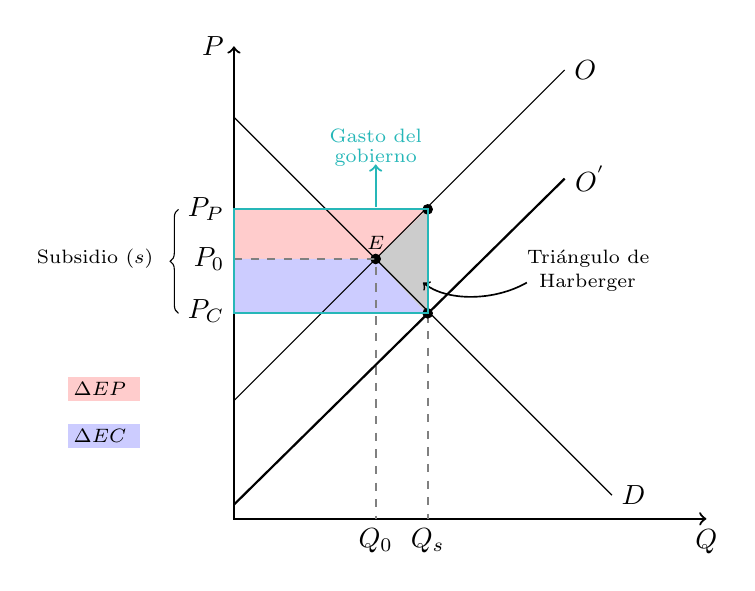
\begin{tikzpicture}[scale=0.6]
\draw[fill,red!20] (0,5.5) -- (0,6.55) -- (4.1,6.55) -- (3,5.5);
\draw[fill,blue!20] (0,5.5) -- (0,4.35) -- (4.1,4.35) -- (3,5.5);
\draw[fill,black!20] (4.1,6.55)--(4.1,4.35)--(3,5.5);
\node [right] at (6,5.5) {\scriptsize Triángulo de};
\node [right] at (6.25,5) {\scriptsize Harberger};
\draw[semithick, <-] (4,5)..controls (4.5,4.6) and (5.5,4.6)..(6.2,5);

\draw[thick,<->] (0,10) node[left]{$P$}--(0,0)--(10,0) node[below]{$Q$};
%\node [below left] at (0,0) {$0$};
\node [below] at (3,0) {{$Q_0$}};
\draw[fill] (3,5.5) circle [radius =0.1] node[above] {\scriptsize $E$};
\node [left] at (0,5.5) {$P_0$};
\node [left] at (0,6.55) {$P_P$};
\node [left] at (0,4.4) {$P_C$};
\node [below] at (4.1,0) {{$Q_s$}};
%\node [below] at (5.25,0) {150};
\draw[thick,gray, dashed](0,6.55)--(4.1,6.55)--(4.1,0);
\draw[thick,gray, dashed](0,4.35)--(4.1,4.35);

\draw [thin,decorate,decoration={brace,amplitude=3pt},xshift=5pt,yshift=0pt](-1.35,4.35) -- (-1.35,6.55);
\draw (-1.5,5.5) node[left]{{\scriptsize Subsidio ($s$)}};

\draw[fill] (4.1,6.55) circle [radius =0.1] ;
\draw[fill] (4.1,4.35) circle [radius =0.1] ;
\draw[thick,gray, dashed](0,5.5)--(3,5.5)--(3,0);
\draw[thin](0,8.5)--(8,0.5) node[right] {$D$};
\draw[black, domain=0:7] plot (\x, {2.5+\x}) node[right] {$O$};

\draw[thick](0,0.3)--(7,7.2) node[right] {$O^{'}$};

\draw [color=BlueGreen, thick] (0,6.55) rectangle (4.1,4.35);
\draw[thick,->, BlueGreen] (3,6.6) -- (3, 7.5);
\node [above, BlueGreen] at (3,7.75) {\scriptsize Gasto del};
\node [above, BlueGreen] at (3,7.25) {\scriptsize gobierno};

\draw[fill,red!20] (-3.5,3) rectangle (-2,2.5); 
\node [right] at (-3.6,2.75) {\scriptsize $\Delta EP$};

\draw[fill,blue!20] (-3.5,2) rectangle (-2,1.5); 
\node [right] at (-3.6,1.75) {\scriptsize $\Delta EC$};

\end{tikzpicture}
\end{figure} 
\end{frame}

\begin{frame}{Distorsiones al equilibrio de mercado}
    En muchas ocasiones el mercado no funciona tan perfectamente. Puede haber dos tipos de distorsiones: \vspace{1mm}
    \begin{itemize}
        \item Creadas por el hombre:
        \begin{itemize}
            \item Monopolios artificiales (escribanos, low cost, SUBE)
             \vspace{1mm}
             \item Impuestos
             \vspace{1mm}
            \item \textbf{Precios máximos o mínimos} (cepo, "Precios Justos")
             \vspace{1mm}
            \item Regulación (ley de alquileres)
        \end{itemize}
        \vspace{1mm}
        \item Por las características de la realidad:
        \begin{itemize}
            \item Monopolios naturales (red eléctrica, agua, gas)   
             \vspace{1mm}
            \item Externalidades (vacunación, contaminación)
             \vspace{1mm}
            \item Bienes públicos
            \vspace{1mm}
            \item Problemas de información
            \begin{itemize}
                \item Atributos ocultos (selección adversa)
                 \vspace{1mm}
                \item Acciones ocultas (moral hazard o riesgo moral)
            \end{itemize}        
        \end{itemize}
    \end{itemize}
\end{frame}

\begin{frame}{Precios máximos}
    \begin{itemize}
        \item Un precio máximo es un límite legal que el gobierno impone para vender un bien.
        \item Para que tenga sentido, este ``tope'' de precio debe estar por debajo del equilibrio de mercado. 
        \item Genera un exceso de demanda.
        \item Doble perjuicio:
            \begin{itemize}
            \item Reduce la cantidad producida
            \item Incentivan a los vendedores a retirar parte de producción del mercado oficia y venderlos más caros en el mercado paralelo $\rightarrow$ si esto sucede, fracasó el objetivo de bajar el precio y ocurrió exactamente lo contrario.
            \end{itemize}
    \end{itemize}
\end{frame}


\begin{frame}{Precio Máximo}
    \begin{figure} [H]
    \centering
    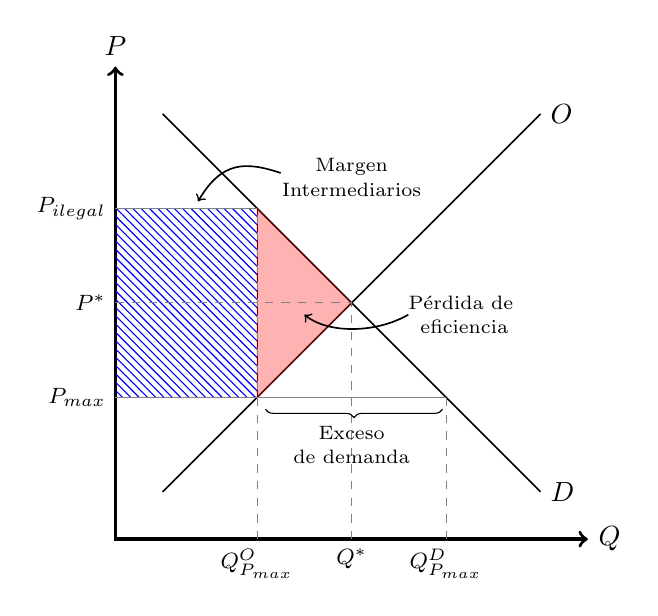
\begin{tikzpicture}[scale=0.6]
    \draw[very thick,<->] (0,10) node[above]{$P$}--(0,0)--(10,0) node[right]{$Q$};
    \draw[semithick](1,1)--(9,9) node[right]{$O$};
    \draw [semithick] (1,9)--(9,1) node[right]{$D$};
    \draw [pattern=north west lines, pattern color=blue] (0,3) rectangle (3,7);
    \filldraw [color=red, opacity=0.3] (3,3) -- (3,7) -- (5,5) -- cycle;
    \node [right] at (6,5) {\scriptsize Pérdida de};
    \node [right] at (6.25,4.5) {\scriptsize eficiencia};
    \draw[semithick, <-] (4,4.75)..controls (4.5,4.35) and (5.5,4.35)..(6.2,4.75);
    \draw[thin, gray, dashed](3,0)--(3,7) ;
    \draw[semithick, gray](0,3)--(7,3);
    \draw[thin, gray, dashed](5,0)--(5,5) ;
    \draw[thin, gray, dashed](0,5)--(5,5) ;
    \draw[thin, gray, dashed](7,0)--(7,3) ;
    \draw[semithick, gray](0,7)--(3,7);
    %\draw[semithick, gray,dashed](3,3)--(7.5,3);
    \node[left] at (0,3){\footnotesize $P_{max}$};
    \node[left] at (0,7){\footnotesize $P_{ilegal}$};
    \node[left] at (0,5){\footnotesize $P^*$};
    \node[below] at (5,0){\footnotesize $Q^*$};
    \node[below] at (3,0){\footnotesize $Q_{P_{max}}^{O}$};
    \node[below] at (7,0){\footnotesize $Q_{P_{max}}^{D}$};
    \draw[semithick, <-] (1.75,7.15).. controls (2.25,8) and (2.75,8).. (3.5,7.75);
    \node[above] at (5,7.5) {\scriptsize Margen};
    \node[above] at (5,7.05) {\scriptsize Intermediarios};
    \draw [thin,decorate,decoration={brace,amplitude=3pt, mirror},xshift=5pt,yshift=0pt](3,2.75) -- (6.75,2.75);
    \draw (5,2.25) node[]{\scriptsize Exceso};
    \draw (5,1.75) node[]{\scriptsize de demanda};
    \end{tikzpicture}
    \label{fig:20.6}
    \end{figure}  
\end{frame}

\begin{frame}{Precio mínimo o precio sostén}
    \begin{itemize}
        \item Un precio mínimo es una medida que el gobierno impone cuando quiere que un precio esté por encima del precio competitivo. \vspace{1mm}
        \item Para que tenga sentido, este ``piso'' de precio debe estar por encima del equilibrio de mercado. \vspace{1mm}
        \item Genera un exceso de oferta.\vspace{1mm}
        \item Los efectos de un precio mínimo dependerán de si:
            \begin{itemize}
            \item Se puede establecer o no un mercado paralelo.
            \item El gobierno decide o no adquirir el excedente.
            \end{itemize}
    \end{itemize}
\end{frame}
    
    
\begin{frame}{Precio mínimo}
\begin{figure} [H]
\centering
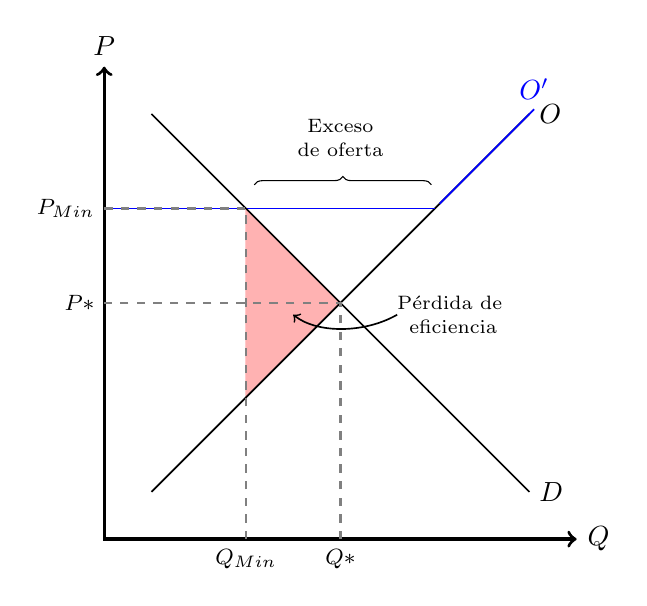
\begin{tikzpicture}[scale=0.6]
\draw[very thick,<->] (0,10) node[above]{$P$}--(0,0)--(10,0) node[right]{$Q$};
\draw[fill,red!30] (5,5)--(3,7)--(3,3);
\node [right] at (6,5) {\scriptsize Pérdida de};
\node [right] at (6.25,4.5) {\scriptsize eficiencia};
\draw[semithick, <-] (4,4.75)..controls (4.5,4.35) and (5.5,4.35)..(6.2,4.75);
\draw [semithick](1,1)--(9,9) node[right]{$O$};
\draw [semithick, blue](7.1,7.1)--(9.1,9.1) node[above]{$O'$};
\draw [semithick, blue](7,7)--(0,7);
\draw [semithick](1,9)--(9,1) node[right]{$D$};
\draw[thick, gray, dashed](3,0)--(3,7) ;
\draw[thick, gray, dashed](0,7)--(3,7) ;
\draw[thick, gray, dashed](5,0)--(5,5)--(0,5) ;
%\node[left] at (0,3){\footnotesize $P^{'}_D$};
\node[left] at (0,7){\footnotesize $P_{Min}$};
\node[below] at (3,0){\footnotesize $Q_{Min}$};
\node[left] at (0,5){\footnotesize $P*$};
\node[below] at (5,0){\footnotesize $Q*$};
\draw [thin,decorate,decoration={brace,amplitude=3pt},xshift=5pt,yshift=0pt](3,7.5) -- (6.75,7.5);
\draw (5,8.75) node[]{\scriptsize Exceso};
\draw (5,8.25) node[]{\scriptsize de oferta};
\end{tikzpicture}
\label{fig:20.7}
\end{figure} 
\end{frame}
    
\begin{frame}{Precio mínimo con mercado paralelo}
\begin{figure} [H]
\centering
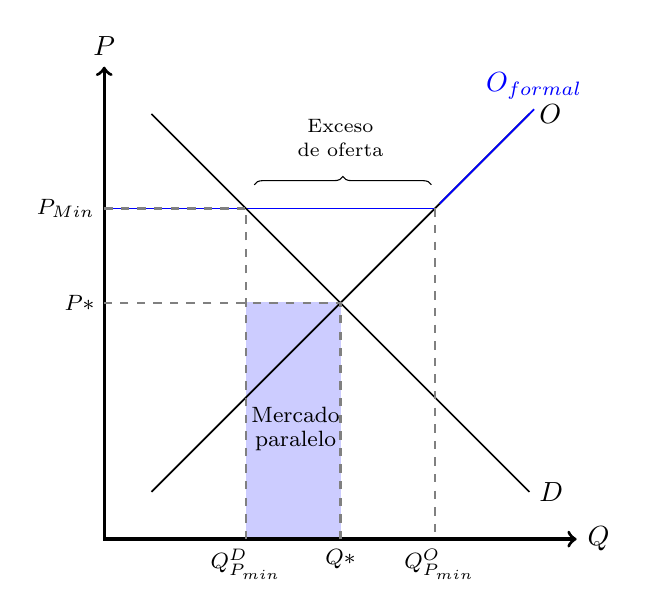
\begin{tikzpicture}[scale=0.6]
\draw[very thick,<->] (0,10) node[above]{$P$}--(0,0)--(10,0) node[right]{$Q$};
\draw[fill,blue!20] (3,0.05)--(5,0.05)--(5,5)--(3,5);
\draw [semithick](1,1)--(9,9) node[right]{$O$};
\draw [semithick, blue](7.1,7.1)--(9.1,9.1) node[above]{$O_{formal}$};
\draw [semithick, blue](7,7)--(0,7);
\draw [semithick](1,9)--(9,1) node[right]{$D$};
\draw[thick, gray, dashed](3,0)--(3,7) ;
\draw[thick, gray, dashed](0,7)--(3,7) ;
%\draw[thick, gray, dashed](0,7)--(7,7)--(7,3)--(0,3) ;
\draw[thick, gray, dashed](5,0)--(5,5)--(0,5) ;
\draw[thick, gray, dashed](7,7)--(7,0) ;
%\node[left] at (0,3){\footnotesize $P^{'}_D$};
\node[left] at (0,7){\footnotesize $P_{Min}$};
\node[below] at (3,0){\footnotesize $Q_{P_{min}}^{D}$};
\node[below] at (7.1,0){\footnotesize $Q_{P_{min}}^{O}$};
\node[left] at (0,5){\footnotesize $P*$};
\node[below] at (5,0){\footnotesize $Q*$};
\node[below] at (4.05,3){\footnotesize Mercado};
\node[below] at (4.05,2.5){\footnotesize paralelo};
\draw [thin,decorate,decoration={brace,amplitude=3pt},xshift=5pt,yshift=0pt](3,7.5) -- (6.75,7.5);
\draw (5,8.75) node[]{\scriptsize Exceso};
\draw (5,8.25) node[]{\scriptsize de oferta};
\end{tikzpicture}
\label{fig:20.7b}
\end{figure}  
\end{frame}
    
\begin{frame}{Precio mínimo con adquisición del excedente}

\begin{columns}
\begin{column}{0.47\textwidth}
\centering
\begin{figure} [H]
\caption{Sin reventa}
\centering
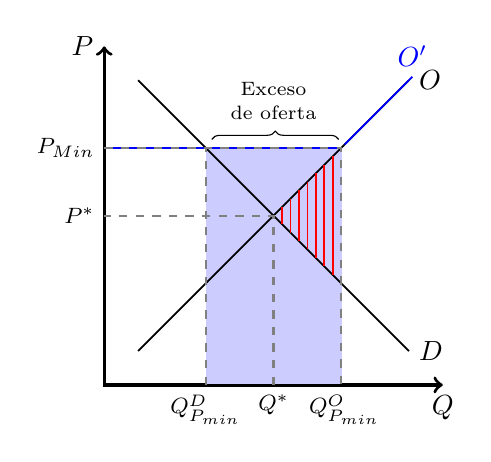
\begin{tikzpicture}[scale=0.43]
\draw[very thick,<->] (0,10) node[left]{$P$}--(0,0)--(10,0) node[below]{$Q$};
\draw[fill,blue!20] (3,0.05)--(7,0.05)--(7,7)--(3,7);
\draw [semithick](1,1)--(9,9) node[right]{$O$};
\draw [semithick, blue](7.1,7.1)--(9.1,9.1) node[above]{$O'$};
\draw [semithick, blue](7,7)--(0,7);
\draw [semithick](1,9)--(9,1) node[right]{$D$};
\draw[semithick, red] (6.75,3.25)--(6.75,6.75);
\draw[semithick, red] (6.5,3.5)--(6.5,6.5);
\draw[semithick, red] (6.25,3.75)--(6.25,6.25);
\draw[semithick, red] (6,4)--(6,6);
\draw[semithick, red] (5.75,4.25)--(5.75,5.75);
\draw[semithick, red] (5.5,4.5)--(5.5,5.5);
\draw[semithick, red] (5.25,4.75)--(5.25,5.25);
%\draw[thick, gray, dashed](2,0)--(2,7) ;
\draw[thick, gray, dashed](0,7)--(2,7) ;
\draw[thick, gray, dashed](0,7)--(7,7)--(7,0) ;
\draw[thick, gray, dashed](5,0)--(5,5)--(0,5) ;
\draw[thick, gray, dashed](3,0)--(3,7);
\node[left] at (0,7){\footnotesize $P_{Min}$};
\node[below] at (3,0){\footnotesize $Q_{P_{min}}^{D}$};
\node[below] at (7.1,0){\footnotesize $Q_{P_{min}}^{O}$};
\node[left] at (0,5){\footnotesize $P^*$};
\node[below] at (5,0){\footnotesize $Q^*$};
\draw [thin,decorate,decoration={brace,amplitude=3pt},xshift=5pt,yshift=0pt](3,7.25) -- (6.75,7.25);
\draw (5,8.75) node[]{\scriptsize Exceso};
\draw (5,8.05) node[]{\scriptsize de oferta};
\end{tikzpicture}
\end{figure} 
\end{column}

\hfill

\begin{column}{0.5\textwidth}
\begin{figure} [H]
\caption{Con reventa}
\centering
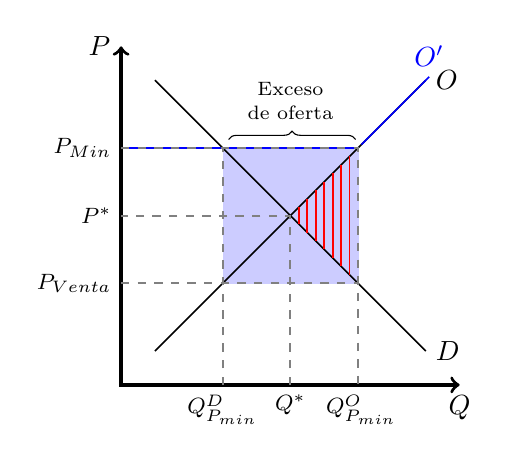
\begin{tikzpicture}[scale=0.43]
\draw[very thick,<->] (0,10) node[left]{$P$}--(0,0)--(10,0) node[below]{$Q$};
\draw[fill,blue!20] (3,3)--(7,3)--(7,7)--(3,7);
\draw [semithick](1,1)--(9,9) node[right]{$O$};
\draw [semithick, blue](7.1,7.1)--(9.1,9.1) node[above]{$O'$};
\draw [semithick, blue](7,7)--(0,7);
\draw [semithick](1,9)--(9,1) node[right]{$D$};
\draw[semithick, red] (6.75,3.25)--(6.75,6.75);
\draw[semithick, red] (6.5,3.5)--(6.5,6.5);
\draw[semithick, red] (6.25,3.75)--(6.25,6.25);
\draw[semithick, red] (6,4)--(6,6);
\draw[semithick, red] (5.75,4.25)--(5.75,5.75);
\draw[semithick, red] (5.5,4.5)--(5.5,5.5);
\draw[semithick, red] (5.25,4.75)--(5.25,5.25);
%\draw[thick, gray, dashed](2,0)--(2,7) ;
\draw[thick, gray, dashed](0,7)--(2,7) ;
\draw[thick, gray, dashed](0,7)--(7,7)--(7,0) ;
\draw[thick, gray, dashed](5,0)--(5,5)--(0,5) ;
\draw[thick, gray, dashed](3,0)--(3,7) ;
\draw[thick, gray, dashed](0,3)--(7,3) ;
%\node[left] at (0,3){\footnotesize $P^{'}_D$};
\node[left] at (0,7){\footnotesize $P_{Min}$};
\node[left] at (0,3){\footnotesize $P_{Venta}$};
\node[below] at (3,0){\footnotesize $Q_{P_{min}}^{D}$};
\node[below] at (7.1,0){\footnotesize $Q_{P_{min}}^{O}$};
\node[left] at (0,5){\footnotesize $P^*$};
\node[below] at (5,0){\footnotesize $Q^*$};
\draw [thin,decorate,decoration={brace,amplitude=3pt},xshift=5pt,yshift=0pt](3,7.25) -- (6.75,7.25);
\draw (5,8.75) node[]{\scriptsize Exceso};
\draw (5,8.05) node[]{\scriptsize de oferta};
\end{tikzpicture}
\end{figure} 
\end{column}
\end{columns}
\end{frame}
    
\begin{frame}{Distorsiones al equilibrio de mercado}
    En muchas ocasiones el mercado no funciona tan perfectamente. Puede haber dos tipos de distorsiones: \vspace{1mm}
    \begin{itemize}
        \item Creadas por el hombre:
        \begin{itemize}
            \item \textbf{Monopolios artificiales} (escribanos, low cost, SUBE)
                \vspace{1mm}
                \item Impuestos
                \vspace{1mm}
            \item Precios máximos o mínimos (cepo, "Precios Justos")
                \vspace{1mm}
            \item Regulación (ley de alquileres)
        \end{itemize}
        \vspace{1mm}
        \item Por las características de la realidad:
        \begin{itemize}
            \item \textbf{Monopolios naturales} (red eléctrica, agua, gas)   
                \vspace{1mm}
            \item Externalidades (vacunación, contaminación)
                \vspace{1mm}
            \item Bienes públicos
            \vspace{1mm}
            \item Problemas de información
            \begin{itemize}
                \item Atributos ocultos (selección adversa)
                    \vspace{1mm}
                \item Acciones ocultas (moral hazard o riesgo moral)
            \end{itemize}        
        \end{itemize}
    \end{itemize}
\end{frame}

\begin{frame}{Monopolios: ¿Cómo regularlos?}
    \begin{itemize}
           \item En general, no es natural que haya un monopolio y la realidad es que la gran mayoría de ellos surgen porque el Estado los crea. 
           \item Sabemos que el monopolio genera una pérdida de eficiencia. 
           \end{itemize}
   \begin{figure} [H]
   \centering
   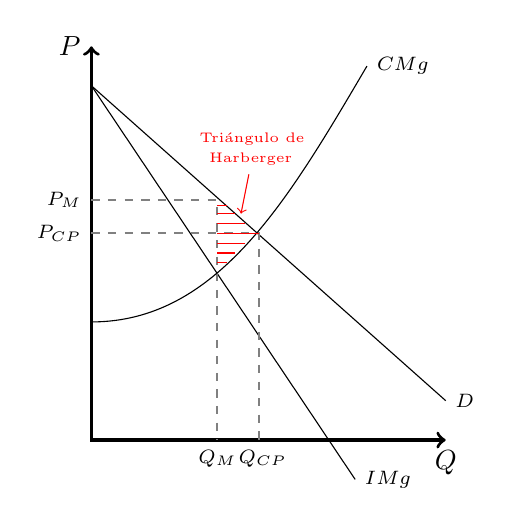
\begin{tikzpicture}[scale=0.5]
   \draw[very thick,<->] (1,10) node[left]{$P$}--(1,0)--(10,0) node[below]{$Q$};
   \draw[thin](1,9)--(10,1) node[right]{\scriptsize $D$};
   \draw[thin](1,9)--(7.7,-1) node[right]{\scriptsize $IMg$};
   \draw[thick,dashed,gray](1,6.1)--(4.2,6.1)--(4.2,0);
   \draw[thick,dashed,gray](1,5.25)--(5.25,5.25)--(5.25,0);
   %\draw(1,1)--(9,9);
   \draw[thin](1,3).. controls (4.2,3) and (6,6.1)..(8,9.5) node[right]{\scriptsize $CMg$};
   \draw[thin, red] (4.2,5.95) to (4.45,5.95) ;
   \draw[thin, red] (4.2,5.75) to (4.65,5.75) ;
   \draw[thin, red] (4.2,5.5) to (4.9,5.5) ;
   \draw[thin, red] (4.2,5.25) to (5.25,5.25) ;
   \draw[thin, red] (4.2,5) to (4.9,5) ;
   \draw[thin, red] (4.2,4.75) to (4.65,4.75) ;
   \draw[thin, red] (4.2,4.5) to (4.45,4.5) ;
   \node [right, red] at (3.5,7.65) {\tiny Triángulo de};
   \node [right, red] at (3.75,7.15) {\tiny Harberger};
   \draw[thin, red,  <-] (4.8,5.75)--(5,6.75);
   \node[below] at(4.2,0) {\scriptsize $Q_M$};
   \node[below] at(5.35,0) {\scriptsize $Q_{CP}$};
   \node[left] at(1,6.1) {\scriptsize $P_{M}$};
   \node[left] at(1,5.25) {\scriptsize $P_{CP}$};
   \end{tikzpicture}
   \end{figure}  
\end{frame}
   
\begin{frame}{Monopolios: ¿Cómo regularlos?}
    \begin{itemize}
       \item Si no se puede desarticular al monopolio, lo ideal sería fijar un precio máximo equivalente al precio de competencia perfecta.
       \item Si el regulador acierta con el precio, el monopolista elegirá producir la cantidad de competencia perfecta y el equilibro eficiente se restituye.
   \end{itemize}
   
   \begin{figure} [H]
       \centering
       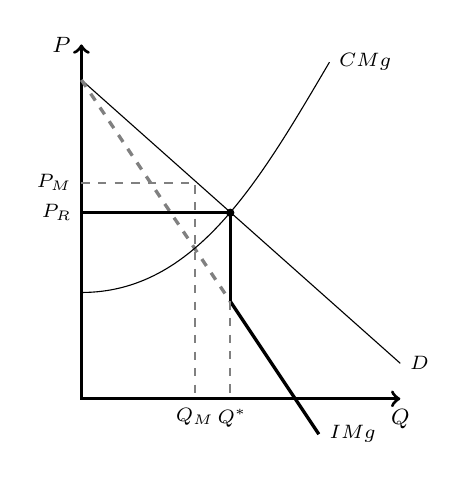
\begin{tikzpicture}[scale=0.45]
       \draw[very thick,<->] (1,10) node[left]{\footnotesize $P$}--(1,0)--(10,0) node[below]{\footnotesize $Q$};
       \draw[thin](1,9)--(10,1) node[right]{\scriptsize  $D$};
       %\draw[thin](1,9)--(7.7,-1) node[right]{$IMg$};
       \draw[very thick,dashed,gray](1,9)--(5.2,2.75);
       \draw[very thick](5.2,2.75)--(7.7,-1) node[right]{\scriptsize $IMg$};
       \draw[thick,dashed,gray](5.2,2.75)--(5.2,0);
       \draw[thick,dashed,gray](1,6.1)--(4.2,6.1)--(4.2,0);
       \draw[very thick](1,5.25)--(5.2,5.25)--(5.2,2.75);
       %\draw(1,1)--(9,9);
       \draw[thin](1,3).. controls (4.2,3) and (6,6.1)..(8,9.5) node[right]{\scriptsize $CMg$};
       \node[below] at(4.2,0) {\scriptsize $Q_M$};
       \node[below] at(5.25,0) {\scriptsize $Q^*$};
       \node[left] at(1,6.1) {\scriptsize $P_{M}$};
       \node[left] at(1,5.25) {\scriptsize $P_{R}$};
       \draw[fill](5.2,5.25) circle [radius =0.1];
       \end{tikzpicture}
   \end{figure} 
\end{frame}
   
\begin{frame}{Regulando un Monopolio Natural}
   \begin{figure} [h!]
   \centering
   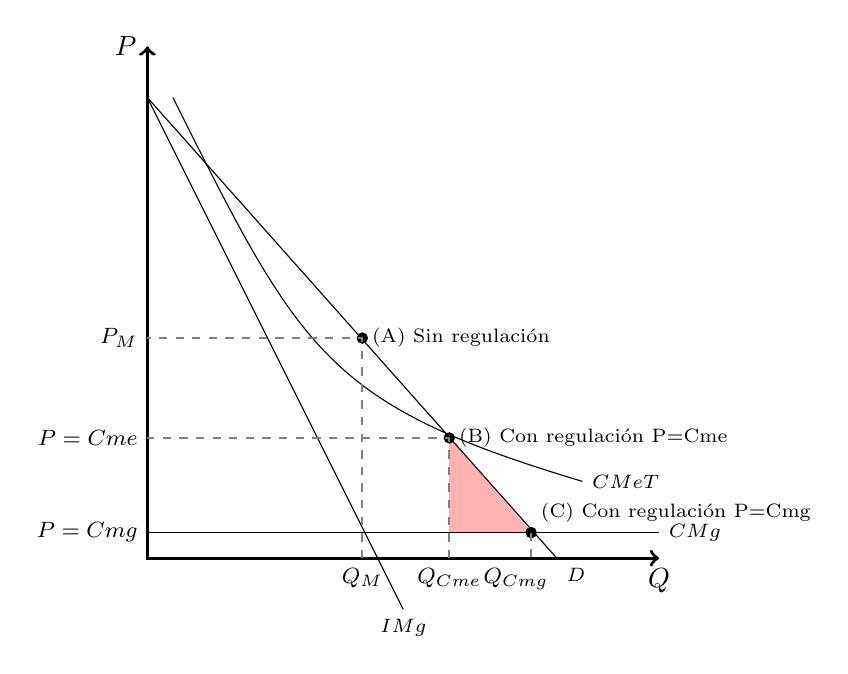
\begin{tikzpicture}[scale=0.65]
   \draw[very thick,<->] (0,10) node[left]{$P$}--(0,0)--(10,0) node[below]{$Q$};
   \draw[fill,red!30] (5.9,0.5)--(5.9,2.35)--(7.5,0.5);
   
   \node[left] at (0,4.3) {\footnotesize $P_M$};
   \node[below] at (4.2,0) {\footnotesize $Q_M$};
   \node[left] at (0,2.35) {\footnotesize $P={Cme}$};
   \node[below] at (5.9,0) {\footnotesize $Q_{Cme}$};
   \node[left] at (0,0.5) {\footnotesize $P={Cmg}$};
   \node[below] at (7.2,0) {\footnotesize $Q_{Cmg}$};
   
   
   \draw[fill] (4.2,4.3) circle [radius =0.1] node[right] {\scriptsize (A) Sin regulación};
   \draw[fill] (5.9,2.35) circle [radius =0.1] node[right] {\scriptsize (B) Con regulación P=Cme};
   \draw[fill] (7.5,0.5) circle [radius =0.1] node[above right] {\scriptsize (C) Con regulación P=Cmg};
   %\draw[fill] (4.2,0.5) circle [radius =0.1] node[above right] {\scriptsize (B)};
   
   \draw[thin](0,9)--(8,0) node[below right]{\scriptsize $D$};
   \draw[thin](0,9)--(5,-1) node[below]{\scriptsize $IMg$};
   \draw[thin](0,0.5)--(10,0.5) node[right]{\scriptsize $CMg$};
   \draw[thin](0.5,9) ..controls (3,4) and (3.5,3) .. (8.5,1.5) node[right]{\scriptsize $CMeT$};
   
   \draw[thick, dashed,gray] (4.2,0)--(4.2,4.3)--(0,4.3);
   \draw[thick, dashed,gray] (5.9,0)--(5.9,2.35)--(0,2.35);
   \draw[thick, dashed,gray] (7.5,0.5)--(7.5,0);
   
   \end{tikzpicture}
   \end{figure} 
\end{frame}
   
\begin{frame}{Monopolio natural eficiente: Poniéndole precio a una carretera}
   \begin{figure} [H]
   \centering
   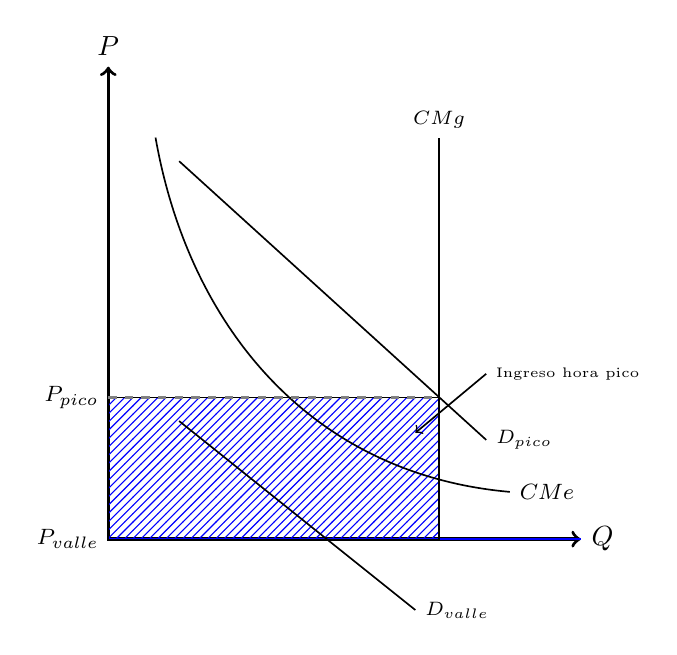
\begin{tikzpicture}[scale=0.6]
   \draw[very thick,<->] (0,10) node[above]{$P$}--(0,0)--(10,0) node[right]{$Q$};
   \draw[semithick, blue] (0,0)--(10,0);
   
   \draw [pattern=north east lines, pattern color=blue] (0,0) rectangle (7,3);
   
   \draw [semithick] (1,8.5) to [out=280,in=175] (8.5,1)node [right] {\footnotesize $CMe$};
   \draw [semithick] (7,0) to (7,8.5);
   \node[above] at (7,8.5) {\scriptsize $CMg$};
   \draw [semithick] (8,2.1) node [right]  {\scriptsize$D_{pico}$} to (1.5,8);
   \draw [semithick] (6.5,-1.5) node [right]  {\scriptsize$D_{valle}$} to (1.5,2.5);
   \draw[thick, gray, dashed](0,3)--(7,3) ;
   \node[left] at (0,3){\footnotesize $P_{pico}$};
   \node[left] at (0,0){\footnotesize $P_{valle}$};
   \draw[semithick, ->] (8,3.5)--(6.5,2.25);
   \node[right] at (8,3.5) {\tiny Ingreso hora pico};
   \end{tikzpicture}
   \label{fig:20.7}
   \end{figure} 
    
\end{frame}

\end{document}
